\documentclass[a4paper]{scrreprt}

% Uncomment to optimize for double-sided printing.
% \KOMAoptions{twoside}

% Set binding correction manually, if known.
% \KOMAoptions{BCOR=2cm}

% Localization options
\usepackage[english]{babel}
\usepackage[T1]{fontenc}
\usepackage[utf8]{inputenc}

% Quotations
\usepackage{dirtytalk}

% Floats
\usepackage{float}

% Enhanced verbatim sections. We're mainly interested in
% \verbatiminput though.
\usepackage{verbatim}

% Automatically remove leading whitespace in lstlisting
\usepackage{lstautogobble}

% PDF-compatible landscape mode.
% Makes PDF viewers show the page rotated by 90°.
\usepackage{pdflscape}

% Advanced tables
\usepackage{array}
\usepackage{tabularx}
\usepackage{longtable}

% Fancy tablerules
\usepackage{booktabs}

% Graphics
\usepackage{graphicx}

% Current time
\usepackage[useregional=numeric]{datetime2}

% Float barriers.
% Automatically add a FloatBarrier to each \section
\usepackage[section]{placeins}

% Custom header and footer
\usepackage{fancyhdr}

\usepackage{geometry}
\usepackage{layout}

% Math tools
\usepackage{mathtools}
% Math symbols
\usepackage{amsmath,amsfonts,amssymb}
\usepackage{amsthm}
% General symbols
\usepackage{stmaryrd}

% Utilities for quotations
\usepackage{csquotes}

% Bibliography
\usepackage[
  style=alphabetic,
  backend=biber, % Default backend, just listed for completness
  sorting=ynt % Sort by year, name, title
]{biblatex}
\addbibresource{references.bib}

\DeclarePairedDelimiter\abs{\lvert}{\rvert}
\DeclarePairedDelimiter\norm{\lVert}{\rVert}
\DeclarePairedDelimiter\floor{\lfloor}{\rfloor}

% Bullet point
\newcommand{\tabitem}{~~\llap{\textbullet}~~}

\pagestyle{plain}
% \fancyhf{}
% \lhead{}
% \lfoot{}
% \rfoot{}
% 
% Source code & highlighting
\usepackage{listings}

% SI units
\usepackage[binary-units=true]{siunitx}
\DeclareSIUnit\cycles{cycles}

\newcommand{\lecture}{61062 - Computer Vision}
\newcommand{\series}{01}
% Convenience commands
\newcommand{\mailsubject}{\lecture - Practical \series}
\newcommand{\maillink}[1]{\href{mailto:#1?subject=\mailsubject}
                               {#1}}

% Should use this command wherever the print date is mentioned.
\newcommand{\printdate}{\today}

\subject{\lecture}
\title{Practical \series}
\subtitle{Report}

\author{Michael Senn \maillink{michael.senn@students.unibe.ch} --- 16-126-880}

\date{\printdate}

% Needs to be the last command in the preamble, for one reason or
% another. 
\usepackage{hyperref}

\begin{document}
\maketitle


\setcounter{chapter}{\numexpr \series - 1 \relax}

\chapter{Practical - Report}

For the whole report, assume that we are working on a $m \times n$ image with
the first dimension being its width. We define indices the way they are
commonly defined for 2D matrices, starting at $(0, 0)$ in the top left, the
first coordinate indicating the row, the second coordinate indicating the
column.

As an example, a $4 \times 3$ image would have the following pixels:
\[
		\begin{bmatrix}
				a_{0, 0} & a_{0, 1} & a_{0, 2} & a_{0, 3} \\
				a_{1, 0} & a_{1, 1} & a_{1, 2} & a_{1, 3} \\
				a_{2, 0} & a_{2, 1} & a_{1, 2} & a_{2, 3}
		\end{bmatrix}
\]

\section{Derivative of the data term}

Starting with the provided discretization of the data term:
\[
		\abs*{u \times k - g}^2 = \sum_{i=0}^{m-1} \sum_{j=0}^{n-1} \abs*{g[i, j] - \sum_{p=0}^{1} \sum_{q=0}^{1} k[p, q] \cdot u[i - p + 1, j - q + 1]}_2^2
\]

We simplify the data term by substituting the assigned blur kernel $k_0$:
\[
		k_0 \coloneqq \begin{bmatrix}
				\frac{1}{2} & \frac{1}{2} \\
				0 & 0
		\end{bmatrix}
\]

\begin{align*}
		D[u] & \coloneqq \abs*{u \times k_0 - g}^2 \\ 
			 & = \sum_{i=0}^{m-1} \sum_{j=0}^{n-1} \abs*{g[i, j] - \frac{1}{2} \cdot (u[i + 1, j + 1] + u[i + 1, j])}_2^2 \\
			 & = \sum_{i=0}^{m-1} \sum_{j=0}^{n-1} \left(g[i, j] - \frac{1}{2} \cdot (u[i + 1, j + 1] + u[i + 1, j])\right)^2
\end{align*}

Where the second simplification is due to the $l_2$ norm of a scalar being
equal to the absolute value of a scalar --- and the square of a real value
being equal to its absolute square. We denote this kernel-specific data term as
$D[u]$ to abbreivate notation. Let further $f(i, j)$ denote the summand:

\begin{align*}
		f(i, j) & \coloneqq \left(g[i, j] - \frac{1}{2} \cdot (u[i + 1, j + 1] + u[i + 1, j])\right)^2
\end{align*}

\subsection{Cases for partial derivation}

We now observe where factors of $u[i, j]$ appear in the expansion of the sum
$D[u]$, to determine the different cases relevant for the differentiation. Note
that there are four possible cases, visualized in figure
\ref{fig:data_term_derivatives}

\begin{figure}
		\centering
		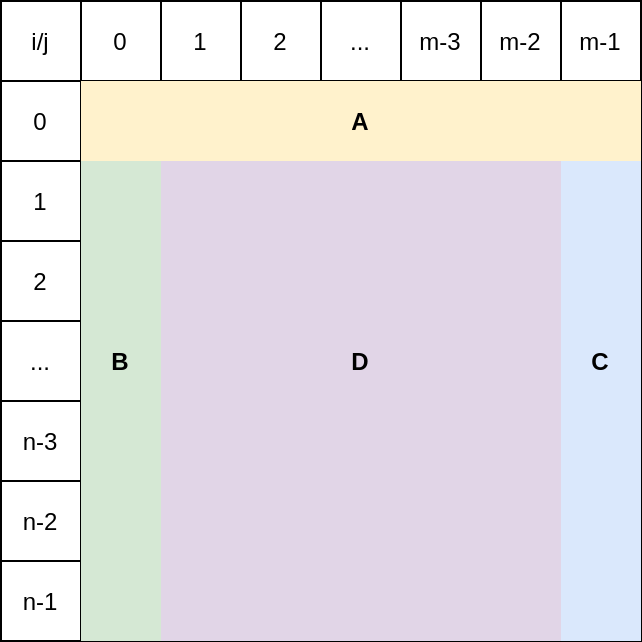
\includegraphics[width=0.6\textwidth]{resources/data_term_derivatives.png}
		\caption{Regions of derivatives of data term}
		\label{fig:data_term_derivatives}
\end{figure}


\subsubsection{Case \emph{A}}

For $i = 0$, none of the factors of the sum will take on the form $u[i, j]$, so
the derivative is a constant $0$:

\[
		\nabla_{D, A} \coloneqq 0
\]


\subsubsection{Case \emph{B}}

For $1 \leq i \leq n-1$, $j = 0$, the factors of the sum will take on the form
$u[i, j]$ for $f(i - 1, j)$. As such:

\begin{align*}
		\nabla_{D, B} \coloneqq \frac{\partial D[u]}{\partial u[i, j]} = \frac{\partial f(i - 1, j)}{\partial u[i, j]}
\end{align*}


\subsubsection{Case \emph{C}}

For $1 \leq i \leq n-1$, $j = m - 1$, the factors of the sum will take on the form
$u[i, j]$ for $f(i - 1, j - 1)$. As such:

\begin{align*}
		\nabla_{D, C} \coloneqq \frac{\partial D[u]}{\partial u[i, j]} = \frac{\partial f(i - 1, j - 1)}{\partial u[i, j]}
\end{align*}


\subsubsection{Case \emph{D}}

For $1 \leq i \leq n-1$, $1 \leq j \leq m - 2$, the factors of the sum will
take on the form $u[i, j]$ for $f(i - 1, j)$ and $f(i - 1, j - 1)$. As such:

\begin{align*}
		\nabla_{D, D} \coloneqq \frac{\partial D[u]}{\partial u[i, j]} = \frac{\partial f(i - 1, j)}{\partial u[i, j]} + \frac{\partial f(i - 1, j - 1)}{\partial u[i, j]}
\end{align*}

\subsection{Determining the derivatives}

We now determine the partial derivatives for $u[i, j]$ of $f(i - 1, j - 1)$ and
$f(i - 1, j)$, using basic laws for derivatives.

\begin{align*}
		\frac{\partial f(i - 1, j)}{\partial u[i, j]} & =
		\frac{1}{2} \cdot u[i, j + 1] + \frac{1}{2} \cdot u[i, j] - g[i - 1, j] \\
		\frac{\partial f(i - 1, j - 1)}{\partial u[i, j]} & =
		\frac{1}{2} \cdot u[i, j - 1] + \frac{1}{2} \cdot u[i, j] - g[i - 1, j - 1]
\end{align*}

Then the derivatives for the four cases above follow directly:

\subsubsection{Case \emph{A}}

\[
		\nabla_{D, A} = 0
\]

\subsubsection{Case \emph{B}}

\[
		\nabla_{D, B} = 
		\frac{1}{2} \cdot u[i, j + 1] + \frac{1}{2} \cdot u[i, j] - g[i - 1, j],
\]

\subsubsection{Case \emph{C}}

\[
		\nabla_{D, C} = 
		\frac{1}{2} \cdot u[i, j - 1] + \frac{1}{2} \cdot u[i, j] - g[i - 1, j - 1]
\]

\subsubsection{Case \emph{D}}

\[
		\nabla_{D, D} = 
		  \frac{1}{2} \cdot u[i, j + 1] + \frac{1}{2} \cdot u[i, j] - g[i - 1, j] + \frac{1}{2} \cdot u[i, j - 1] + \frac{1}{2} \cdot u[i, j] - g[i - 1, j - 1]
\]

\section{Derivative of Gaussian prior}

Starting with the provided discretization of the Gaussian prior, adjusted for a
$m \times n$ image:

\begin{align*}
		G[u] & \coloneqq \sum_{i=0}^{n-2} \sum_{j=0}^{m-2} \left((u[i + 1, j] - u[i, j])^2 + (u[i,j + 1] - u[i, j])^2\right) \\
			 & + \sum_{i=0}^{n-2} \left((u[i + 1, m - 1] - u[i, m - 1])^2\right) \\
			 & + \sum_{j=0}^{m-2} \left((u[n - 1, j + 1] - u[n - 1, j])^2\right)
\end{align*}

Let $f(\hat{i}, \hat{j})$ denote the summand of $G[u]$ for $i = \hat{i}, j =
\hat{j}$.  That is:

\begin{align*}
		f(i, j) \coloneqq 
		\begin{cases}
				(u[i + 1, j] - u[i, j])^2 + (u[i, j + 1] - u[i, j])^2, & i \in [0, n - 2], j \in [0, m - 2] \\
				(u[i + 1, m - 1] - u[i, m - 1])^2, & i \in [0, n - 2], j = m - 1 \\
				(u[n - 1, j + 1] - u[n - 1, j])^2, & i = n - 1, j \in [0, m - 2]
		\end{cases}
\end{align*}

\subsection{Cases for partial derivation}

We now observe where factors of $u[i, j]$ appear in the expansion of the sum
$G[u]$, to determine the different cases relevant for the differentiation. Note
that there are eight possible cases, visualized in figure
\ref{fig:gaussian_prior_derivatives}

\begin{figure}
		\centering
		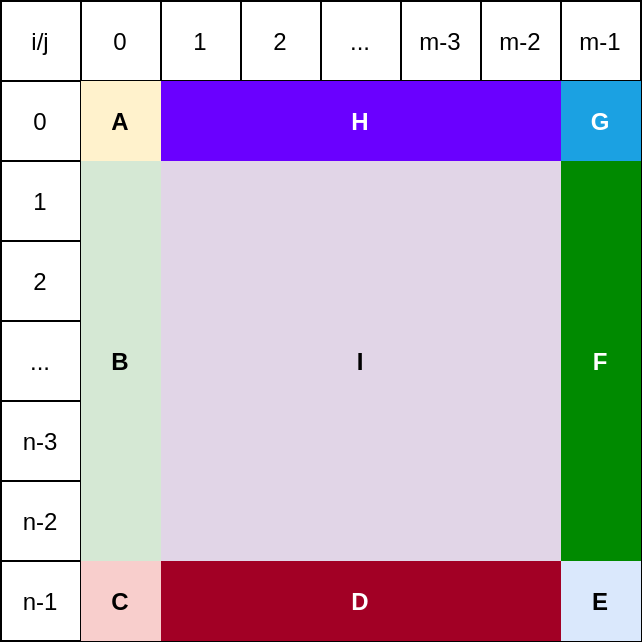
\includegraphics[width=0.6\textwidth]{resources/gaussian_prior_derivatives.drawio.png}
		\caption{Regions of derivatives of gaussian prior}
		\label{fig:gaussian_prior_derivatives}
\end{figure}


\subsubsection{Case \emph{A}}

For $i = j = 0$, the factors of the sum will take on the form $u[i, j]$ for
$f(i, j)$. As such:

\begin{align*}
		\nabla_{G, A} \coloneqq \frac{\partial G[u]}{\partial u[i, j]} = 
		  \frac{\partial f(i, j)}{\partial u[i, j]}
\end{align*}

\subsubsection{Case \emph{B}}

For $1 \leq i \leq n - 2$, $j = 0$, the factors of the sum will take on the
form $u[i, j]$ for $f(i - 1, j)$ and $f(i, j)$. As such:

\begin{align*}
		\nabla_{G, B} \coloneqq \frac{\partial G[u]}{\partial u[i, j]} = 
		  \frac{\partial f(i - 1, j)}{\partial u[i, j]} 
		  + \frac{\partial f(i, j)}{\partial u[i, j]}
\end{align*}

\subsubsection{Case \emph{C}}

For $i = n - 1$, $j = 0$, the factors of the sum will take on the form $u[i,
j]$ for $f(i - 1, j)$ and $f(i, j)$. As such:

\begin{align*}
		\nabla_{G, C} \coloneqq \frac{\partial G[u]}{\partial u[i, j]} = 
		  \frac{\partial f(i - 1, j)}{\partial u[i, j]} 
		  + \frac{\partial f(i, j)}{\partial u[i, j]}
\end{align*}

\subsubsection{Case \emph{D}}

For $i = n - 1$, $1 \leq j \leq m - 2$, the factors of the sum will take on the
form $u[i, j]$ for $f(i - 1, j)$, $f(i, j - 1)$ and $f(i, j)$. As such:

\begin{align*}
		\nabla_{G, D} \coloneqq \frac{\partial G[u]}{\partial u[i, j]} = 
		  \frac{\partial f(i - 1, j)}{\partial u[i, j]} 
		  + \frac{\partial f(i, j - 1)}{\partial u[i, j]} 
		  + \frac{\partial f(i, j)}{\partial u[i, j]}
\end{align*}

\subsubsection{Case \emph{E}}

For $i = n - 1$, $j = m - 1$, the factors of the sum will take on the form
$u[i, j]$ for $f(i - 1, j)$ and $f(i, j - 1)$. As such:

\begin{align*}
		\nabla_{G, E} \coloneqq \frac{\partial G[u]}{\partial u[i, j]} = 
		  \frac{\partial f(i - 1, j)}{\partial u[i, j]}
		  + \frac{\partial f(i, j - 1)}{\partial u[i, j]}
\end{align*}

\subsubsection{Case \emph{F}}

For $1 \leq i \leq n - 2$, $j = m - 1$, the factors of the sum will take on the
form $u[i, j]$ for $f(i - 1, j)$, $f(i, j - 1)$ and $f(i, j)$. As such:

\begin{align*}
		\nabla_{G, F} \coloneqq \frac{\partial G[u]}{\partial u[i, j]} = 
		  \frac{\partial f(i - 1, j)}{\partial u[i, j]}
		  + \frac{\partial f(i, j - 1)}{\partial u[i, j]}
		  + \frac{\partial f(i, j)}{\partial u[i, j]}
\end{align*}

\subsubsection{Case \emph{G}}

For $i = 0$, $j = m -1$, the factors of the sum will take on the form $u[i, j]$
for $f(i, j - 1)$ and $f(i, j)$. As such:

\begin{align*}
		\nabla_{G, G} \coloneqq \frac{\partial G[u]}{\partial u[i, j]} = 
		  \frac{\partial f(i, j - 1)}{\partial u[i, j]}
		  + \frac{\partial f(i, j)}{\partial u[i, j]}
\end{align*}

\subsubsection{Case \emph{H}}

For $i = 0$, $1 \leq j \leq m - 2$, the factors of the sum will take on the
form $u[i, j]$ for $f(i, j - 1)$ and $f(i, j)$. As such:

\begin{align*}
		\nabla_{G, H} \coloneqq \frac{\partial G[u]}{\partial u[i, j]} = 
		  \frac{\partial f(i, j - 1)}{\partial u[i, j]}
		  + \frac{\partial f(i, j)}{\partial u[i, j]}
\end{align*}

\subsubsection{Case \emph{I}}

For $1 \leq i \leq n - 2$, $1 \leq j \leq m - 2$, the factors of the sum will
take on the form $u[i, j]$ for $f(i - 1, j)$, $f(i, j - 1)$ and $f(i, j)$. As
such:

\begin{align*}
		\nabla_{G, I} \coloneqq \frac{\partial G[u]}{\partial u[i, j]} = 
		  \frac{\partial f(i - 1, j)}{\partial u[i, j]}
		  + \frac{\partial f(i, j - 1)}{\partial u[i, j]}
		  + \frac{\partial f(i, j)}{\partial u[i, j]}
\end{align*}

\subsection{Determining the derivatives}

We now determine the partial derivatives for $u[i, j]$ of $f(i - 1, j)$, $f(i,
j - 1)$ and $f(i, j)$, using basic laws for derivatives.

\begin{align*}
		\frac{\partial f(i - 1, j)}{\partial u[i, j]} & =
		  2 \cdot u[i, j] - 2 \cdot u[i - 1, j] \\
		\frac{\partial f(i, j - 1)}{\partial u[i, j]} & =
		  2 \cdot u[i, j] - 2 \cdot u[i, j - 1] \\
		\frac{\partial f(i, j)}{\partial u[i, j]} & =
		  \begin{cases}
				  4 \cdot u[i, j] - 2 \cdot u[i + 1, j] - 2 \cdot u[i, j + 1] 
				    & i \in [0, n - 2], j \in [0, m - 2] \\
				  2 \cdot u[i, j] - 2 \cdot u[i + 1, j] 
				    & i \in [0, n - 2], j = m - 1 \\
				  2 \cdot u[i, j] - 2 \cdot u[i, j + 1] 
					& i = n - 1, j \in [0, m - 2]
		  \end{cases} \\
\end{align*}

Then the derivatives for the eight cases above follow directly:

\subsubsection{Case \emph{A}}

\begin{align*}
		\nabla_{G, A} = 
		  4 \cdot u[i, j] - 2 \cdot u[i + 1, j] - 2 \cdot u[i, j + 1]
\end{align*}

\subsubsection{Case \emph{B}}

\begin{align*}
		\nabla_{G, B} = 
		  6 \cdot u[i, j] - 2 \cdot u[i - 1, j] - 2 \cdot u[i + 1, j] - 2 \cdot u[i, j + 1]
\end{align*}

\subsubsection{Case \emph{C}}

\begin{align*}
		\nabla_{G, C} =
		  4 \cdot u[i, j] - 2 \cdot u[i - 1, j] - 2 \cdot u[i, j + 1]
\end{align*}

\subsubsection{Case \emph{D}}

\begin{align*}
		\nabla_{G, D} = 
		  6 \cdot u[i, j] - 2 \cdot u[i - 1, j] - 2 \cdot u[i, j - 1] - 2 \cdot u[i, j + 1]
\end{align*}

\subsubsection{Case \emph{E}}

\begin{align*}
		\nabla_{G, E} =
		  4 \cdot u[i, j] - 2 \cdot u[i - 1, j] - 2 \cdot u[i, j - 1]
\end{align*}

\subsubsection{Case \emph{F}}

\begin{align*}
		\nabla_{G, F} =
		  6 \cdot u[i, j] - 2 \cdot u[i, j - 1] - 2 \cdot u[i + 1, j] - 2 \cdot u[i - 1, j]
\end{align*}

\subsubsection{Case \emph{G}}

\begin{align*}
		\nabla_{G, G} = 
		  4 \cdot u[i, j] - 2 \cdot u[i, j - 1] - 2 \cdot u[i + 1, j]
\end{align*}

\subsubsection{Case \emph{H}}

\begin{align*}
		\nabla_{G, H} =
		  6 \cdot u[i, j] - 2 \cdot u[i + 1, j] - 2 \cdot u[i, j + 1] - 2 \cdot u[i, j - 1]
\end{align*}

\subsubsection{Case \emph{I}}

\begin{align*}
		\nabla_{G, I} =
		  8 \cdot u[i, j] - 2 \cdot u[i + 1, j] - 2 \cdot u[i, j + 1] - 2 \cdot u[i - 1, j] - 2 \cdot u[i, j - 1]
\end{align*}


\section{Discretization of anisotropic prior}

\section{Derivative of anisotropic prior}

\section{Gradient of energy term}

\printbibliography

\end{document}
